%==============================================================================
%  TRIPTERON - Delivery 1 : Design proposal (corrected English edition)
%  IM0240 Machine Design I - Universidad EAFIT
%==============================================================================
\documentclass[11pt]{article}
\usepackage[english]{babel}
\usepackage[utf8]{inputenc}
\usepackage{lmodern}
\usepackage[T1]{fontenc}
\usepackage{amsmath,amssymb,bm}
\usepackage{graphicx}
\usepackage{booktabs}
\usepackage{longtable}
\usepackage{array}
\usepackage{placeins}
\usepackage{lastpage}
\usepackage{enumitem}
\usepackage{siunitx}
\usepackage{tikz}
\usetikzlibrary{arrows.meta,positioning,shapes.geometric,calc}
\usepackage[table]{xcolor}
\usepackage[left=2.3cm,right=2.3cm,top=3.2cm,bottom=2.5cm]{geometry}
\usepackage{fancyhdr}
\usepackage[hidelinks]{hyperref}
\usepackage{titlesec}
\sisetup{detect-all, per-mode=symbol}

\definecolor{eafitblue}{HTML}{16436f}
\definecolor{lightgray}{HTML}{f0efe9}

\titleformat{\section}{\normalfont\large\bfseries\color{eafitblue}}{\thesection.}{0.6em}{}[{\titlerule[0.6pt]}]
\titleformat{\subsection}{\normalfont\normalsize\bfseries}{\thesubsection.}{0.6em}{}
\setlength{\parskip}{4pt}
\setlength{\parindent}{0pt}

\pagestyle{fancy}\fancyhf{}
\renewcommand{\headrulewidth}{0.4pt}
\fancyhead[L]{\small\textsc{Tripteron CNC router -- Design proposal}}
\fancyhead[R]{\small IM0240 Machine Design I}
\fancyfoot[C]{\small\thepage\ / \pageref{LastPage}}

\begin{document}

%------------------------------------------------------------------ cover
\thispagestyle{empty}
\begin{center}
\vspace*{1cm}
{\Large\scshape Universidad EAFIT}\\[3pt]
{\large School of Applied Sciences and Engineering}\\[3pt]
{\large Department of Mechanical Engineering}\\[3pt]
{\large IM0240 -- Machine Design I}\\[1.8cm]

{\color{eafitblue}\rule{\textwidth}{1.4pt}}\\[12pt]
{\huge\bfseries Design proposal for a}\\[6pt]
{\huge\bfseries CNC router machine}\\[10pt]
{\LARGE Tripteron 3-PRRR architecture}\\[10pt]
{\large\bfseries Delivery 1 -- Corrected English edition}\\[8pt]
{\color{eafitblue}\rule{\textwidth}{1.4pt}}\\[2cm]

{\large\bfseries Group 2}\\[8pt]
{\large David Amell Osorio}\\[4pt]
{\large Ronny Antonio Bueno}\\[4pt]
{\large Juan Jos\'e Garc\'ia}\\[4pt]
{\large Germ\'an Gabriel Ria\~no Barrera}\\[4pt]
{\large Sebasti\'an Rinc\'on Mart\'inez}\\[4pt]
{\large Juan Manuel Rodr\'iguez Duque}\\[4pt]
{\large David Zuluaga Henao}\\[1.4cm]

{\large\bfseries Course lecturer}\\[8pt]
{\large Juan Andr\'es Gallego S\'anchez}

\vfill
{\large Medell\'in, Colombia -- 11 February 2024}
\end{center}

\clearpage
\tableofcontents
\clearpage

%==============================================================================
\section{Introduction}
%==============================================================================

Within the Machine Design course, the assignment is to conceive, design and build a CNC
router that satisfies a specific set of technical requirements. The goal is a machine
that, using the concepts studied in the course, can be adapted to the manufacturing
processes where light routing and engraving are needed.

This document is the first delivery of the project. It defines the problem, surveys the
state of the art, establishes the requirements and the product design specification,
compares the mechanism architectures that could satisfy them and justifies the
architecture that was selected: a \textbf{Tripteron}, a three-degree-of-freedom
translational parallel machine with three PRRR legs actuated by power screws.

This is a corrected and restructured English edition of the original proposal. The
technical content of the original has been preserved; the errors identified in it are
listed and corrected in Section~\ref{sec:corrections}.

%==============================================================================
\section{Brief}
%==============================================================================

\subsection{What is a router machine?}

A CNC router is an automated machine that uses computer numerical control to cut, carve or
engrave materials such as wood, plastic, metal and composites. It works with a rotating
cutting tool --- an end mill --- whose path is controlled by a program. Because the
process is both precise and repeatable, routers are a basic tool in manufacturing and
design workshops.

\subsection{How does it work?}

The tool moves in a three-dimensional coordinate system driven by three motors. The
operator's controller commands the motors so that the tool sweeps the programmed path
inside the working volume. Each motor drives one power screw, and each power screw moves
one axis of the machine.

\subsection{Which materials are viable for its construction?}

Different parts call for different materials:

\begin{center}
\begin{tabular}{@{}l>{\raggedright\arraybackslash}p{4.0cm}>{\raggedright\arraybackslash}p{8.4cm}@{}}
\toprule
\textbf{Part} & \textbf{Material} & \textbf{Reason} \\
\midrule
External enclosure & PVC or wood & Carries no significant load; low cost, easy to shape \\
Structural frame   & Steel or aluminium & Carries the machining loads and the weight of the drives \\
Mechanism (links, screws) & Steel & Stiffness and wear resistance govern the accuracy \\
\bottomrule
\end{tabular}
\end{center}

%==============================================================================
\section{Objectives}
%==============================================================================

\subsection{General objective}

Design and build a numerically controlled router able to cut at least \SI{1}{\milli\metre}
of depth in a range of materials, making the best use of the available materials,
manufacturing processes and aesthetics.

\subsection{Specific objectives}

\begin{itemize}[leftmargin=*]
  \item Define the flows through the machine --- the inputs it needs and the outputs it
        must deliver --- so that the concept is built on a solid functional basis.
  \item Develop a support structure that guarantees stable operation, minimising
        vibration and avoiding buckling under the weight of the equipment.
  \item Design a machine that meets the client's expectations in appearance, design and
        aesthetics, so that the result is attractive from the user's point of view.
  \item Plan the specific requirements needed to satisfy the client, ensuring the
        technical and functional feasibility of the project.
  \item Select a kinematic chain and a mechanism that suit both the client's needs and an
        efficient development process, guaranteeing adequate performance.
\end{itemize}

%==============================================================================
\section{State of the art}
%==============================================================================

\subsection{CNC machines}

A CNC (computer numerical control) machine removes the human factor from the trajectory of
the tool: the cut is performed automatically by a computer that feeds numerical
coordinates to the machine, which is what makes millimetre and sub-millimetre precision
repeatable.

\subsection{Motion control}

The motion of a CNC machine is controlled by software that interprets G-code. The general
process is:

\begin{enumerate}[leftmargin=*]
  \item \textbf{Model design.} The part is modelled in 3D with a CAD package.
  \item \textbf{G-code generation.} A CAM package converts the model into the G-code that
        specifies tool movements, cutting speeds and tooling.
  \item \textbf{Transfer.} The program is transferred to the machine over a USB drive or a
        network connection.
  \item \textbf{Set-up.} The tool is mounted, the stock is clamped and the cutting
        parameters --- feed rate and spindle speed --- are configured.
  \item \textbf{Execution.} The controller interprets the G-code and moves the axes
        accordingly, producing the part.
\end{enumerate}

\subsection{The CNC program}

A CNC program is a set of coded instructions written mainly in G-code, complemented by M,
S and T codes depending on the functions the machine offers.

\subsection{Types of CNC machines}

\begin{center}
\begin{tabular}{@{}l>{\raggedright\arraybackslash}p{10.7cm}@{}}
\toprule
\textbf{Criterion} & \textbf{Classes} \\
\midrule
By function & Milling machines, lathes, drilling machines, plasma cutters, grinders. \\
By motion   & \emph{Point to point}: the stock and the tool are positioned and held while
              the cutter completes the operation, then retracted.
              \emph{Contouring}: the tool follows the contour of the part along a
              continuous path. \\
By number of axes & 2 axes; 2.5 axes (the three axes move, but $x$ and $y$ position first
              and only then does $z$ work); 3 axes; 4 axes (3 axes plus one rotation,
              $A$ or $B$); 5 axes (3 axes plus two rotations, $A$ and $B$). \\
\bottomrule
\end{tabular}
\end{center}

The machine of this project is a \textbf{3-axis contouring router}.

\subsection{Applications}

Manufacture of metal and plastic parts; cutting and engraving of wood, metal, plastic and
stone for signage, architectural models and artistic engraving; prototyping and mass
production of identical parts; medical devices, prostheses and surgical instrument
components; and, on machines equipped for it, additive manufacturing.

\subsection{Key components}

\begin{description}[leftmargin=0pt,style=nextline]
  \item[Power screw] A mechanical device that converts rotary into linear motion. A
        threaded screw engages a nut with an internal thread; turning the screw
        translates the nut along its axis. It is the element that turns the rotation of
        the motor into the feed of the axis, and it is sized in Delivery~3.
  \item[NEMA 34 stepper motor] A NEMA standard frame size, roughly \SI{86}{\milli\metre}
        across the body, known for high torque. It is used in industrial CNC machines,
        large-format 3D printers and automation equipment. The closed-loop 86HB250 variant
        selected for this project delivers \SI{4.5}{\newton\metre} of holding torque.
  \item[End mill] The rotating cutting tool. A sharpened metal tip turns at high speed and
        removes material on contact. End mills are interchangeable and are chosen
        according to the material and the finish required.
\end{description}

%==============================================================================
\section{User definition}
%==============================================================================

The user of the router is someone experienced with cutting equipment who is looking for a
versatile, easy to operate and affordable machine. The intended duty is light cutting
without extreme demands, in a workshop with a mains supply. The machine is to be operated
by people of at least 18 years of age.

%==============================================================================
\section{Conceptual design}
%==============================================================================

\subsection{Requirements imposed by the course}

\begin{itemize}[leftmargin=*,nosep]
  \item A cutting machine (router) with \textbf{3 degrees of freedom}.
  \item The machine \textbf{may not} be a cartesian system built from prismatic pairs in
        series.
  \item The degrees of freedom must be \textbf{coupled}, i.e.\ the architecture must be a
        parallel one.
  \item The prismatic pairs must be \textbf{actuated by power screws}.
  \item The machine may be spatial (linear delta or Tripteron) or planar.
  \item It must be able to cut at least \SI{1}{\milli\metre} deep in aluminium, copper,
        brass or nylon.
\end{itemize}

\subsection{Technical design requirements}

\begin{center}
\begin{tabular}{@{}l>{\raggedright\arraybackslash}p{10.4cm}@{}}
\toprule
\textbf{Requirement} & \textbf{Definition} \\
\midrule
Feed rate   & Constant routing speed of approximately \SI{10}{\milli\metre\per\second}. \\
Accuracy    & Path error not greater than \SI{1}{\milli\metre}. \\
Cutting capability & Able to route wood, aluminium, copper, brass and nylon to a depth of at least \SI{1}{\milli\metre}. \\
Safety      & The machine must not put the operator at risk during operation. \\
Control     & The operator must have buttons or instruments to start and stop the process. \\
Energy and information & The machine must carry a control system that transmits accurate
              process information while a stable power supply is guaranteed. \\
\bottomrule
\end{tabular}
\end{center}

\subsection{Black box}

The black box states \emph{what} the machine does without saying \emph{how}: the three
flows --- material, energy and information --- that cross its boundary.

\begin{figure}[htbp]\centering
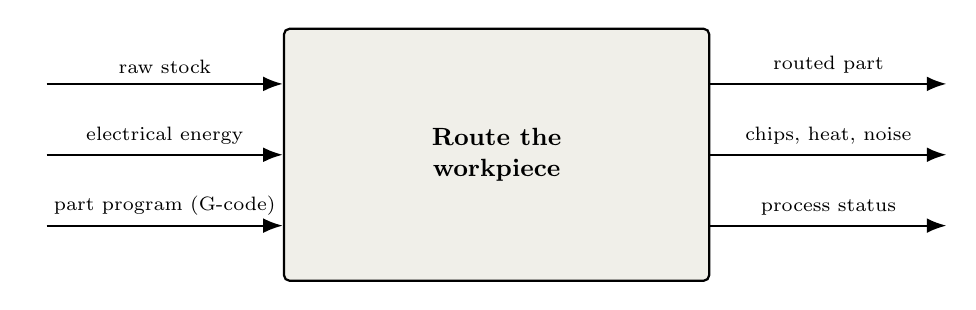
\begin{tikzpicture}[font=\small,node distance=6mm,
  flow/.style={-{Latex[length=2.5mm]},thick}]
\node[draw,fill=lightgray,minimum width=5.4cm,minimum height=3.2cm,align=center,
      rounded corners=2pt,thick] (bb)
      {\bfseries Route the\\\bfseries workpiece};
\node[left=3.0cm of bb.west,anchor=east,align=right] (in) {};
\draw[flow] ($(bb.west)+(-3.0,0.9)$) -- node[above,font=\scriptsize]{raw stock} ($(bb.west)+(0,0.9)$);
\draw[flow] ($(bb.west)+(-3.0,0.0)$) -- node[above,font=\scriptsize]{electrical energy} ($(bb.west)+(0,0.0)$);
\draw[flow] ($(bb.west)+(-3.0,-0.9)$) -- node[above,font=\scriptsize]{part program (G-code)} ($(bb.west)+(0,-0.9)$);
\draw[flow] ($(bb.east)+(0,0.9)$) -- node[above,font=\scriptsize]{routed part} ($(bb.east)+(3.0,0.9)$);
\draw[flow] ($(bb.east)+(0,0.0)$) -- node[above,font=\scriptsize]{chips, heat, noise} ($(bb.east)+(3.0,0.0)$);
\draw[flow] ($(bb.east)+(0,-0.9)$) -- node[above,font=\scriptsize]{process status} ($(bb.east)+(3.0,-0.9)$);
\end{tikzpicture}
\caption{Black box of the router: material, energy and information flows.}
\end{figure}

\subsection{Functional structure}

The functional structure --- the ``transparent box'' --- decomposes the overall function
into the elementary functions that the machine must perform, which is what allows the
concept to be generated function by function instead of by copying an existing machine.

\begin{figure}[htbp]\centering
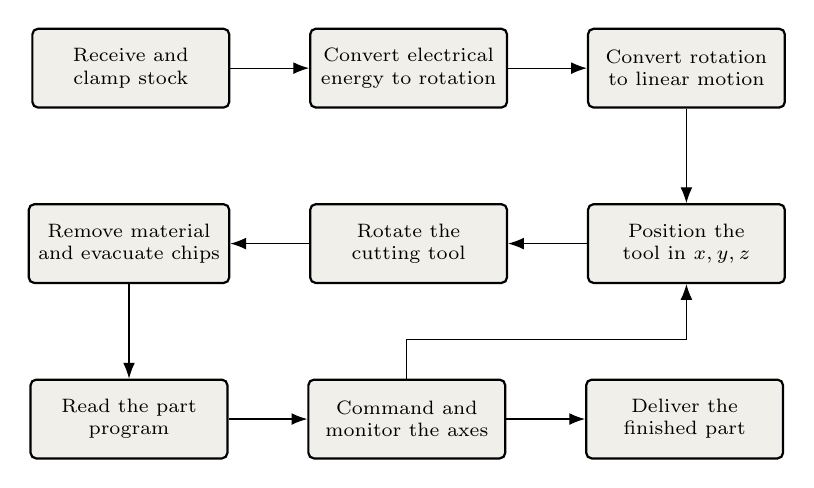
\begin{tikzpicture}[font=\scriptsize,
  fn/.style={draw,fill=lightgray,rounded corners=2pt,minimum width=2.5cm,
             minimum height=1.0cm,align=center,thick},
  flow/.style={-{Latex[length=2mm]}}]
\node[fn] (f1) {Receive and\\clamp stock};
\node[fn,right=1.0cm of f1] (f2) {Convert electrical\\energy to rotation};
\node[fn,right=1.0cm of f2] (f3) {Convert rotation\\to linear motion};
\node[fn,below=1.2cm of f3] (f4) {Position the\\tool in $x,y,z$};
\node[fn,left=1.0cm of f4] (f5) {Rotate the\\cutting tool};
\node[fn,left=1.0cm of f5] (f6) {Remove material\\and evacuate chips};
\node[fn,below=1.2cm of f6] (f7) {Read the part\\program};
\node[fn,right=1.0cm of f7] (f8) {Command and\\monitor the axes};
\node[fn,right=1.0cm of f8] (f9) {Deliver the\\finished part};
\draw[flow] (f1)--(f2); \draw[flow] (f2)--(f3); \draw[flow] (f3)--(f4);
\draw[flow] (f4)--(f5); \draw[flow] (f5)--(f6); \draw[flow] (f6)--(f7);
\draw[flow] (f7)--(f8); \draw[flow] (f8)--(f9);
\draw[flow] (f8.north) -- ++(0,0.5) -| (f4.south);
\end{tikzpicture}
\caption{Functional structure of the machine.}
\end{figure}
\FloatBarrier

\subsection{Attributes}

The attributes are the measurable quantities through which each flow is evaluated in the
product design specification.

\begin{center}
\begin{tabular}{@{}llll@{}}
\toprule
\textbf{Material} & \textbf{On/off} & \textbf{Manual work} & \textbf{Energy} \\
\midrule
Strength        & Production accuracy & Accuracy            & Transfer \\
Specific weight & Power required      & Instructions        & Voltage \\
Size            &                     & Ease of production  & Current \\
Thickness       &                     &                     & Power \\
\bottomrule
\end{tabular}
\end{center}

\subsection{Product design specification (PDS)}

\begin{center}\small
\begin{tabular}{@{}cl l r l c c@{}}
\toprule
\textbf{\#} & \textbf{Requirement} & \textbf{Metric} & \textbf{Value} & \textbf{Unit} & \textbf{Weight} & \textbf{D/d} \\
\midrule
1  & Degrees of freedom      & Coupled DOF        & 3       & DOF        & 4 & D \\
2  & Service life            & Time               & 3       & h          & 4 & d \\
3  & Ease of assembly        & Time               & $<3$    & h          & 4 & D \\
4  & Ease of maintenance     & Time               & 2       & h          & 4 & d \\
5  & Cost                    & Money              & 500\,000& COP        & 5 & D \\
6  & Construction time       & Time               & 3       & months     & 4 & d \\
7  & Width                   & Length             & 0.55    & m          & 5 & d \\
8  & Depth                   & Length             & 0.55    & m          & 5 & d \\
9  & Height                  & Length             & 0.55    & m          & 5 & d \\
10 & Feed rate               & Speed              & 10      & mm/s       & 3 & D \\
11 & Path accuracy           & Length             & $\le 1$ & mm         & 5 & D \\
12 & Depth of cut            & Length             & $\ge 1$ & mm         & 5 & D \\
13 & Emergency stop response & Time               & 0.5     & s          & 6 & D \\
14 & Positioning resolution  & Length             & 0.1     & mm         & 7 & D \\
\bottomrule
\end{tabular}
\end{center}
{\footnotesize D = demand (must be met), d = desire (desirable). The units of rows 10--14
were corrected with respect to the original proposal; see
Section~\ref{sec:corrections}.}

\subsection{Morphological matrix}

Each elementary function of the functional structure was given a set of possible
solutions, and the concepts were generated by combining one solution per function.

\begin{center}\small
\begin{tabular}{@{}l>{\raggedright\arraybackslash}p{3.3cm}>{\raggedright\arraybackslash}p{3.3cm}>{\raggedright\arraybackslash}p{3.3cm}@{}}
\toprule
\textbf{Function} & \textbf{Solution A} & \textbf{Solution B} & \textbf{Solution C} \\
\midrule
Convert energy to rotation & Stepper motor & Servo motor & DC motor with encoder \\
Convert rotation to translation & Power screw & Belt and pulley & Rack and pinion \\
Guide the carriage & Linear rail and bearing block & Round shaft and bushing & Dovetail slide \\
Mechanism architecture & Tripteron (3-PRRR) & Linear delta & Serial cartesian (not allowed) \\
Structure & Welded steel tube frame & Bolted aluminium extrusion & Laser-cut plate \\
Control & Microcontroller with drivers & Industrial CNC controller & PC with parallel port \\
\bottomrule
\end{tabular}
\end{center}

The evaluation of the resulting combinations against the PDS selected: stepper motors,
power screws, linear rails, a welded steel frame, a microcontroller-based controller, and
the \textbf{Tripteron} architecture.

%==============================================================================
\section{Mechanism architecture}
%==============================================================================

\subsection{Topological synthesis}

\begin{description}[leftmargin=0pt,style=nextline]
  \item[Base] The fixed frame. It does not move while the machine is operating and it
        carries the three guides, the three screws and the work table.
  \item[Arms] Three identical legs. Each leg is driven along one axis and transmits that
        motion to the platform through two links and three parallel revolute joints.
  \item[Cutting tool] Mounted on the platform where the three legs meet. It performs the
        milling, drilling or cutting work.
\end{description}

\subsection{Mobility}

The machine has 10 moving bodies --- three carriages, six links and the platform --- and
12 joints, each with one degree of freedom (3 prismatic and 9 revolute). The
Kutzbach--Gr\"ubler criterion for spatial mechanisms gives
\begin{equation}
M = 6\,(n_b) - \sum_{i}(6-f_i) = 6\times10 - 12\times5 = 0 ,
\end{equation}
where $n_b=10$ is the number of moving bodies and $f_i=1$ for every joint.

The formula predicts a structure, yet the machine moves with three degrees of freedom.
The discrepancy is not an error: the Tripteron belongs to the family of
\textbf{over-constrained} mechanisms, in which the special geometry --- the three revolute
axes of each leg parallel to one another and perpendicular to its prismatic axis ---
makes three of the 60 constraint equations redundant. The true mobility is therefore
\begin{equation}
M = 0 + 3 = 3 \quad\text{translations, no rotation.}
\end{equation}
Exactly the same number of redundancies appears again in Delivery~3, where the static
equilibrium system turns out to have 63 unknowns and rank 60. The two analyses are
consistent, and the consequence for manufacturing is important: an over-constrained
machine is sensitive to assembly errors, so the parallelism and squareness tolerances of
the three guides must be tight.

\subsection{Why a Tripteron}

\begin{center}
\begin{tabular}{@{}l>{\raggedright\arraybackslash}p{5.2cm}>{\raggedright\arraybackslash}p{5.2cm}@{}}
\toprule
\textbf{Architecture} & \textbf{Advantages} & \textbf{Disadvantages} \\
\midrule
Serial cartesian & Simple, decoupled, cubic workspace &
                   \textbf{Not allowed by the course}; each axis carries the next \\
Linear delta     & Light moving mass, fast &
                   Coupled kinematics, curved workspace boundary, singularities inside
                   the useful volume \\
\textbf{Tripteron} & \textbf{Decoupled} like a cartesian machine but built as a parallel
                   mechanism; cubic workspace; actuators fixed to the frame; simple
                   controller &
                   Over-constrained, so it demands accurate assembly; more links than a
                   delta \\
\bottomrule
\end{tabular}
\end{center}

The Tripteron was selected because it satisfies the course requirement of coupled,
parallel architecture while keeping the two practical advantages of a cartesian machine:
a cubic workspace and a controller that needs no coordinate transformation. Delivery~3
confirms both properties numerically.

%==============================================================================
\section{Concept proposals}
%==============================================================================

Each member of the team developed an individual concept; the concepts were then compared
against the PDS and merged into a single final concept.

\begin{figure}[htbp]\centering
\begin{minipage}[t]{0.24\textwidth}\centering
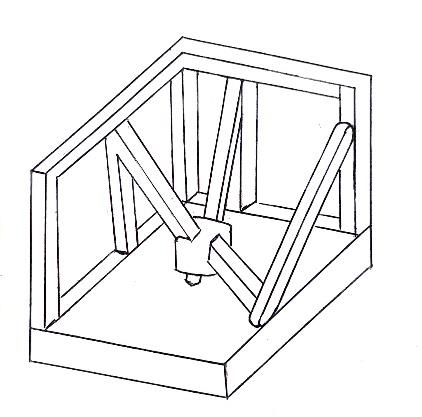
\includegraphics[height=3.0cm,width=\textwidth,keepaspectratio]{figures/concept_amell.png}\\[4pt]{\footnotesize David Amell Osorio}
\end{minipage}\hfill
\begin{minipage}[t]{0.24\textwidth}\centering
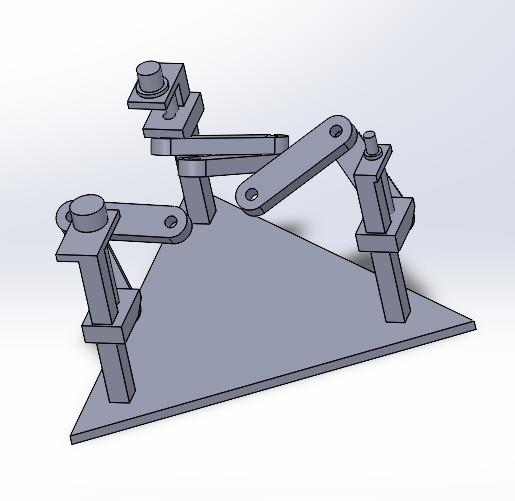
\includegraphics[height=3.0cm,width=\textwidth,keepaspectratio]{figures/concept_bueno.png}\\[4pt]{\footnotesize Ronny Antonio Bueno}
\end{minipage}\hfill
\begin{minipage}[t]{0.24\textwidth}\centering
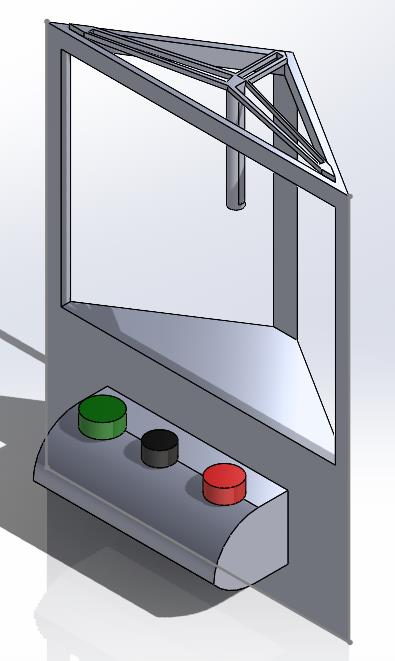
\includegraphics[height=3.0cm,width=\textwidth,keepaspectratio]{figures/concept_garcia.png}\\[4pt]{\footnotesize Juan Jos\'e Garc\'ia}
\end{minipage}\hfill
\begin{minipage}[t]{0.24\textwidth}\centering
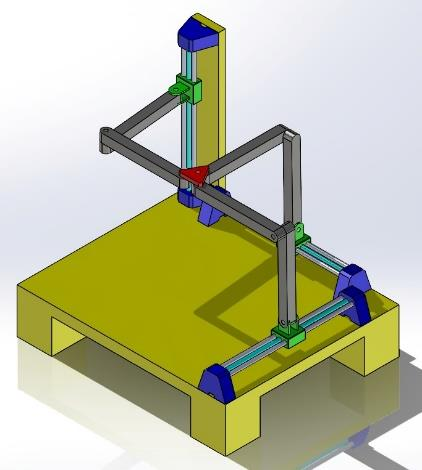
\includegraphics[height=3.0cm,width=\textwidth,keepaspectratio]{figures/concept_riano.png}\\[4pt]{\footnotesize Germ\'an G. Ria\~no}
\end{minipage}

\vspace{10pt}

\begin{minipage}[t]{0.24\textwidth}\centering
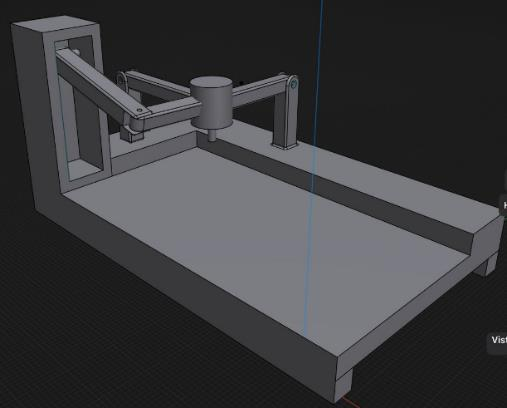
\includegraphics[height=3.0cm,width=\textwidth,keepaspectratio]{figures/concept_rincon.png}\\[4pt]{\footnotesize Sebasti\'an Rinc\'on}
\end{minipage}\hfill
\begin{minipage}[t]{0.24\textwidth}\centering
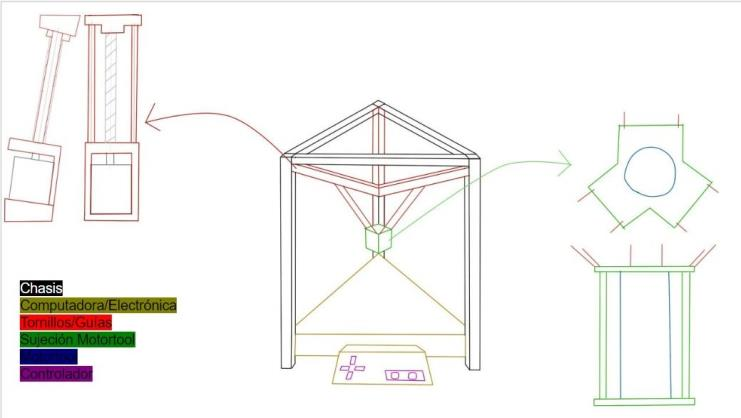
\includegraphics[height=3.0cm,width=\textwidth,keepaspectratio]{figures/concept_rodriguez.png}\\[4pt]{\footnotesize Juan M. Rodr\'iguez}
\end{minipage}\hfill
\begin{minipage}[t]{0.24\textwidth}\centering
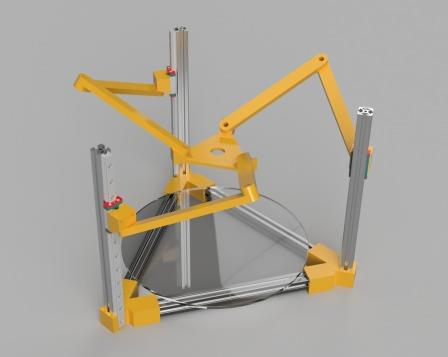
\includegraphics[height=3.0cm,width=\textwidth,keepaspectratio]{figures/concept_zuluaga.png}\\[4pt]{\footnotesize David Zuluaga Henao}
\end{minipage}\hfill
\begin{minipage}[t]{0.24\textwidth}\centering
\rule{0pt}{3.0cm}
\end{minipage}
\caption{The seven individual concepts, one per member of the group.}
\end{figure}

\begin{figure}[htbp]\centering
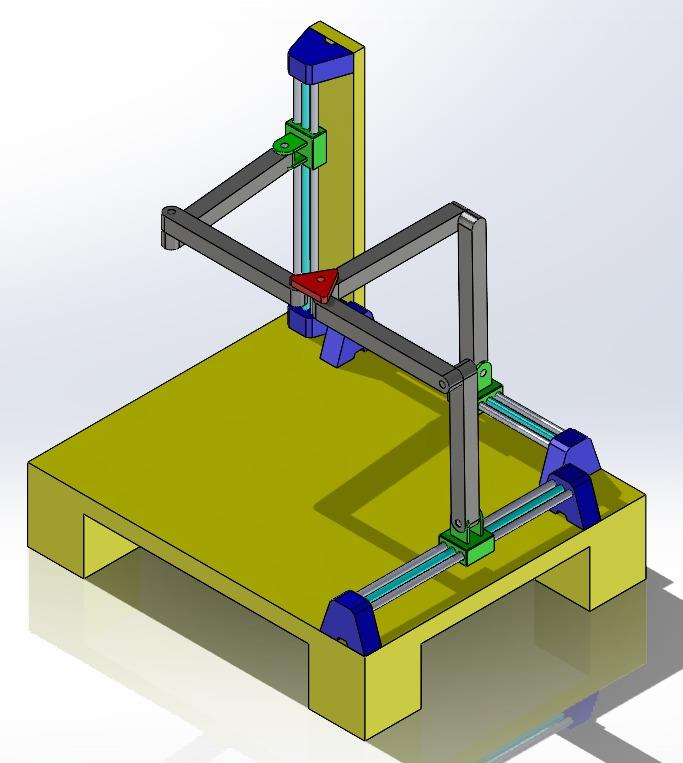
\includegraphics[width=0.52\textwidth]{figures/concept_final.png}
\caption{Final concept: welded frame, three orthogonal screw-driven axes, Tripteron legs
and a spindle mounted on the moving platform.}
\end{figure}
\FloatBarrier

The final concept keeps the vertical axis on a column at the rear of the frame and the two
horizontal axes along the base, so that the three screws are all mounted on the fixed
structure and no motor travels with the tool. The work table is fixed, which removes the
need to accelerate the workpiece.

%==============================================================================
\section{Work methodology}
%==============================================================================

The CNC router is developed as a collaborative effort in which every member of the group
contributes ideas and knowledge. The drawing package is produced jointly, so that
different points of view and experience are integrated into it. The construction of the
machine --- enclosure, structure and mechanism --- is carried out by specialised
sub-groups whose work is then merged in an integration process that ends on 24 May.

Every week the group meets to agree on the tasks to be developed next and to report on
the ones already completed. Working together is what keeps the process on track.

\subsection{Planned dates}

\begin{center}
\begin{tabular}{@{}llll@{}}
\toprule
\textbf{29 July} & \textbf{12 August} & \textbf{16 September} & \textbf{28 October} \\
\midrule
Concept delivery & Drawing delivery & Model delivery & Calculation delivery \\
\bottomrule
\end{tabular}
\end{center}

\subsection{Distribution of the work}

\begin{center}
\begin{tabular}{@{}l>{\raggedright\arraybackslash}p{9.4cm}@{}}
\toprule
\textbf{Member} & \textbf{Responsibility} \\
\midrule
David Amell Osorio        & Tool support, final assembly drawings, kinematic analysis \\
Ronny Antonio Bueno       & Arms and R-pair system, guide calculations \\
Juan Jos\'e Garc\'ia      & Electrical system and wiring, lead-screw calculations \\
Germ\'an G. Ria\~no Barrera & Chassis and guide system, drawings, lead-screw and guide calculations \\
Sebasti\'an Rinc\'on Mart\'inez & Static analysis \\
Juan Manuel Rodr\'iguez Duque   & Guide system drawings, static analysis \\
David Zuluaga Henao       & Kinematics, finite element analysis of the chassis, spacers \\
\bottomrule
\end{tabular}
\end{center}

%==============================================================================
\section{Planned calculations}
%==============================================================================

\begin{itemize}[leftmargin=*,nosep]
  \item A \textbf{kinematic analysis} to obtain the position, velocity and acceleration of
        every body of the machine, and to establish the workspace.
  \item A \textbf{static analysis} to identify the forces on the actuators, the joints and
        the links.
  \item A \textbf{solid mechanics} verification to confirm that the selected materials
        withstand those forces --- in particular the power screws, which are slender and
        loaded in compression.
  \item A \textbf{finite element analysis} of the frame, whose redundant three-dimensional
        structure cannot be resolved by hand.
\end{itemize}

All four were carried out and are reported in Delivery~3.

%==============================================================================
\section{Conclusions}
%==============================================================================

\begin{enumerate}[leftmargin=*]
  \item A Tripteron was selected over a linear delta because it is the only parallel
        architecture that keeps the decoupled behaviour and the cubic workspace of a
        cartesian machine, which simplifies both the control and the programming of the
        part.
  \item The design must be optimised for material usage and cost: the PDS sets a budget of
        COP 500\,000 and an overall size of \SI{0.55}{\metre} per side, and both are
        binding constraints on the frame.
  \item The mobility analysis shows that the machine is over-constrained. This is
        acceptable, but it converts the parallelism of the three guides into a critical
        manufacturing tolerance, and it must be watched during assembly.
  \item The kinematic analysis is required before the structure can be dimensioned, since
        the stroke of each screw and the length of the links determine the size of the
        frame.
\end{enumerate}

%==============================================================================
\section{Corrections with respect to the original proposal}\label{sec:corrections}
%==============================================================================

\begin{center}
\begin{tabular}{@{}c>{\raggedright\arraybackslash}p{4.6cm}>{\raggedright\arraybackslash}p{5.2cm}>{\raggedright\arraybackslash}p{4.2cm}@{}}
\toprule
\textbf{\#} & \textbf{Original} & \textbf{Problem} & \textbf{Correction} \\
\midrule
1 & Mobility computed as $M=3n-2J_1-J_2=3$
  & That is Gr\"ubler's formula for \emph{planar} mechanisms; the Tripteron is spatial.
  & Kutzbach for spatial mechanisms, $M=6n_b-\sum(6-f_i)=0$, plus 3 redundant constraints
    $\Rightarrow M=3$ \\
2 & ``3 DOF: rotation about the base ($z$) and horizontal motion''
  & The Tripteron platform does not rotate; its three degrees of freedom are pure
    translations.
  & 3 translations $x$, $y$, $z$; zero rotations \\
3 & Feed rate listed as ``300 millimetres'' with the metric ``distance''
  & A feed rate is a speed, not a distance; the value contradicted the
    \SI{10}{\milli\metre\per\second} stated in the text.
  & \SI{10}{\milli\metre\per\second} \\
4 & Accuracy listed as ``85 percent''
  & Accuracy of a machine tool is a length, not a percentage.
  & Path error $\le\SI{1}{\milli\metre}$ \\
5 & Cutting capability listed as ``10 cm/s$^2$'', metric ``area/time$^2$''
  & Neither the unit nor the metric corresponds to a depth of cut.
  & Depth of cut $\ge\SI{1}{\milli\metre}$ \\
6 & Service life of 3 hours
  & Three hours is a test duration, not a service life.
  & Retained as stated, but reinterpreted as continuous operating time between maintenance
    stops \\
7 & Section numbering out of step (section 3 containing subsections 4.1, 4.2, \dots)
  & Made cross-referencing impossible.
  & Numbering rebuilt \\
8 & Repeated figures and an unattributed image taken from the internet
  & Duplicated content and unreferenced third-party material.
  & Duplicates removed; only the group's own material is reproduced \\
9 & Planned dates of 29 July, 12 August, 16 September and 28 October
  & They belong to a different semester's calendar: this proposal is dated 11 February
    2024 and the project ran from February to May 2024.
  & The table is kept as submitted; the dates actually met were 11 February (proposal),
    3 March (drawings) and 25 May 2024 (calculations) \\
\bottomrule
\end{tabular}
\end{center}

%==============================================================================
\section{References}
%==============================================================================

\begin{enumerate}[leftmargin=*,nosep]
  \item Gosselin, C.\ et al.\ \textit{The Tripteron: a new 3-DOF translational parallel
        mechanism}. Universit\'e Laval.
  \item RepRap Wiki. \textit{Tripteron}. \url{https://reprap.org/wiki/Tripteron}
  \item O'Connell, J. \textit{Tripteron 3D Printer: All You Need to Know}. All3DP, 2021.
  \item Budynas, R.\ and Nisbett, K. \textit{Shigley's Mechanical Engineering Design},
        10th ed., McGraw-Hill. Chapter 8: power screws.
  \item SIDECO. \textit{\textquotedblleft Qu\'e son las m\'aquinas CNC\textquotedblright}.
        \url{https://sideco.com.mx/que-son-las-maquinas-cnc/}
  \item Aeromaquinados. \textit{M\'aquina CNC}.
        \url{https://aeromaquinados.com/maquina-cnc/}
\end{enumerate}

\end{document}
